\section{Développement}

    \subsection{Chiffrement d'une image}

        \begin{frame}
            \frametitle{Chiffrement par mélange pseudo-aléatoire}
            \centering{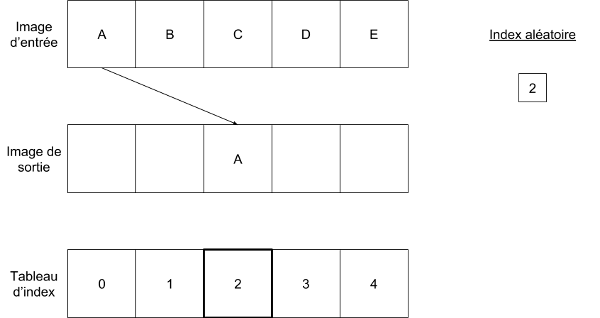
\includegraphics[width=.5\linewidth]{./rsc/index_1_1.png}}
            \pause
            \begin{columns}
                \begin{column}{.45\linewidth}
                    \centering{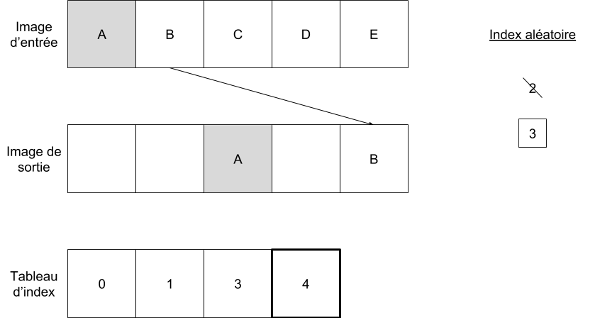
\includegraphics[width=\linewidth]{./rsc/index_1_2.png}}
                \end{column}
                \pause
                \begin{column}{.45\linewidth}
                    \centering{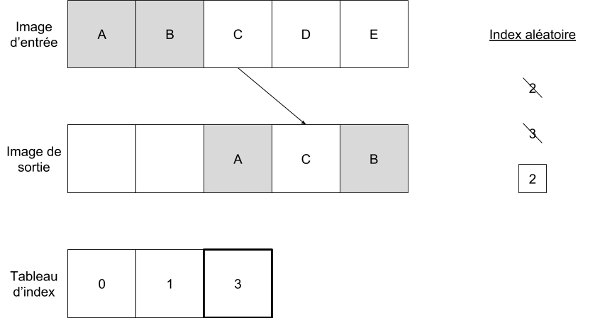
\includegraphics[width=\linewidth]{./rsc/index_1_3.png}}
                \end{column}
            \end{columns}
        \end{frame}

        \begin{frame}
            \frametitle{Déchiffrement par mélange pseudo-aléatoire}
            \centering{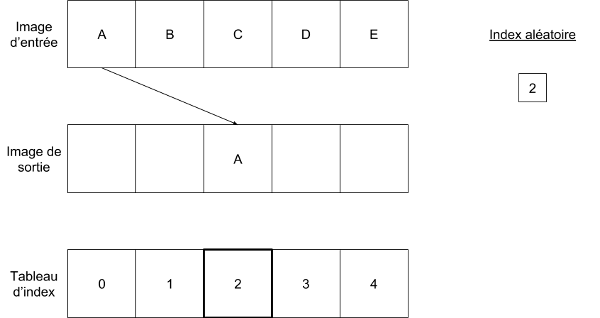
\includegraphics[width=.5\linewidth]{./rsc/index_1_1.png}}
            \pause
            \begin{columns}
                \begin{column}{.45\linewidth}
                    \centering{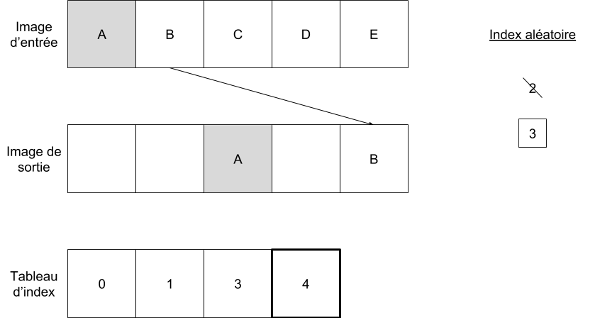
\includegraphics[width=\linewidth]{./rsc/index_1_2.png}}
                \end{column}
                \pause
                \begin{column}{.45\linewidth}
                    \centering{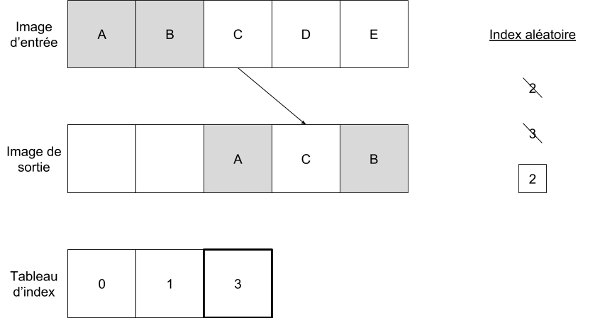
\includegraphics[width=\linewidth]{./rsc/index_1_3.png}}
                \end{column}
            \end{columns}
        \end{frame}

    \subsection{Lecture d'une image}

        \begin{frame}
            \frametitle{Prétraitement}
            \framesubtitle{Niveau de gris / Binaire}
            \begin{columns}
                \begin{column}{.3\linewidth}
                    \centering{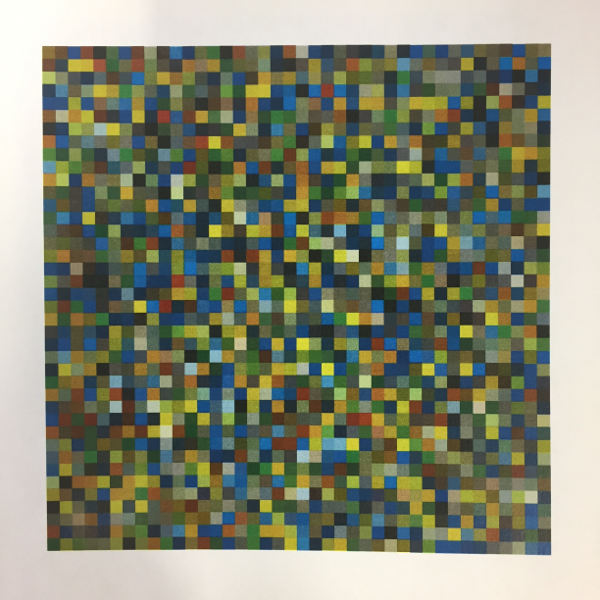
\includegraphics[width=\linewidth]{./rsc/40.png}}
                \end{column}
                \pause
                \begin{column}{.3\linewidth}
                    \centering{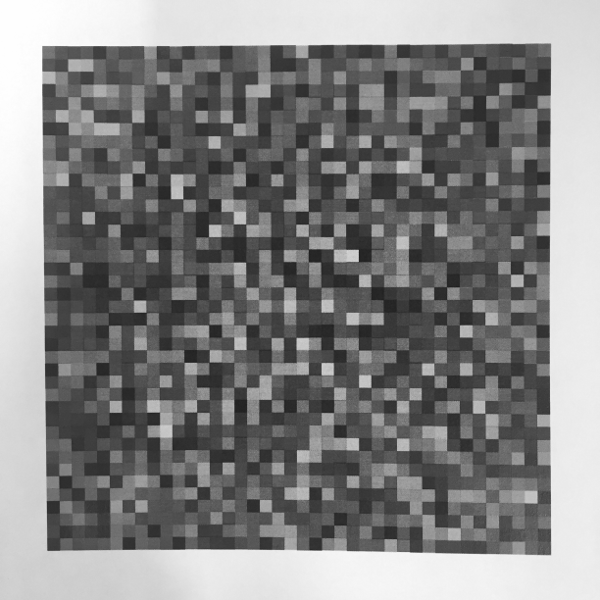
\includegraphics[width=\linewidth]{./rsc/gray_scale.png}}
                \end{column}
                \pause
                \begin{column}{.3\linewidth}
                    \centering{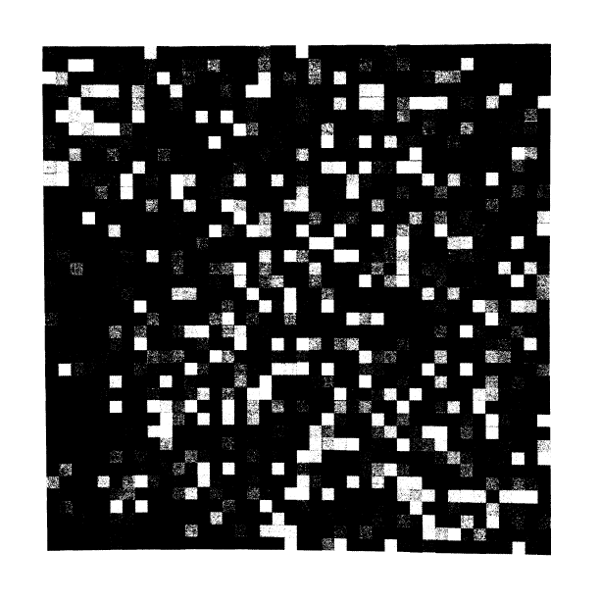
\includegraphics[width=\linewidth]{./rsc/binary.png}}
                \end{column}
            \end{columns}
            \pause
            \centering{x*r + y*G + z*B}\\
            \centering{seuil = moyenne luminance}
        \end{frame}

        \begin{frame}
            \frametitle{Prétraitement}
            \framesubtitle{Détection des angles / Transformation}
            \begin{columns}
                \begin{column}{.3\linewidth}
                    \centering{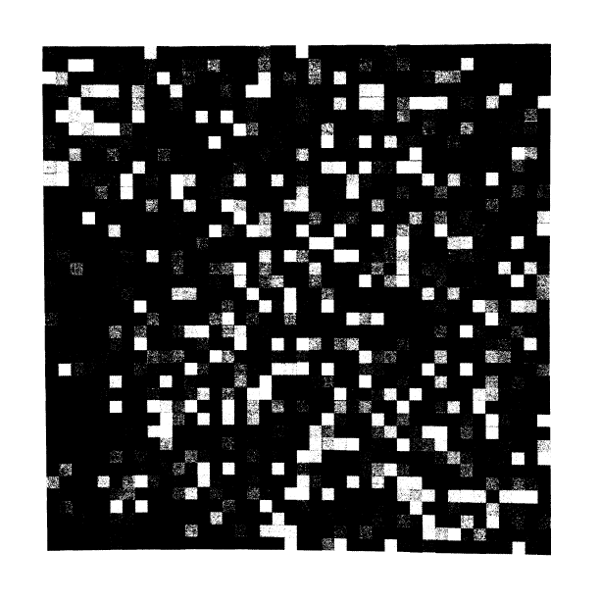
\includegraphics[width=\linewidth]{./rsc/binary.png}}
                \end{column}
                \pause
                \begin{column}{.3\linewidth}
                    \centering{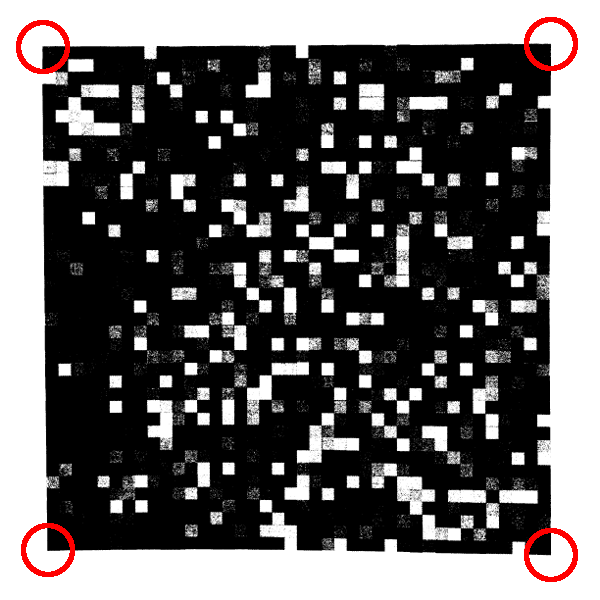
\includegraphics[width=\linewidth]{./rsc/angles.png}}
                \end{column}
                \pause
                \begin{column}{.3\linewidth}
                    \centering{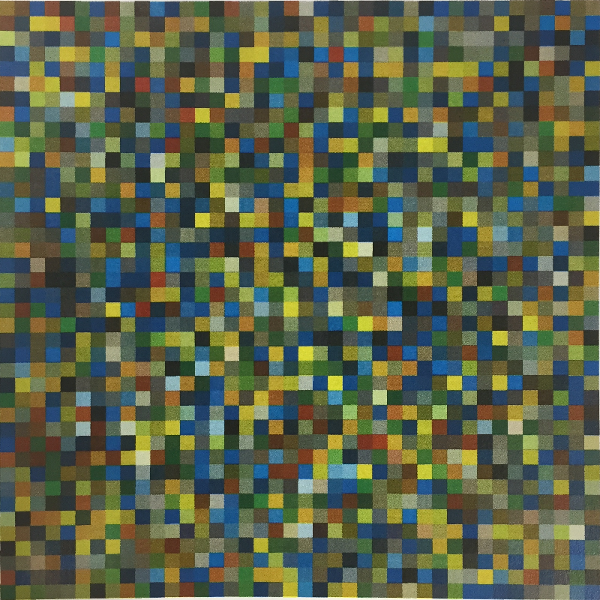
\includegraphics[width=\linewidth]{./rsc/transform.png}}
                \end{column}
            \end{columns}
            \pause
            \centering{x*r + y*G + z*B}\\
            \centering{seuil = moyenne luminance}\\
            \centering{x*r + y*G + z*B}\\
            \centering{seuil = moyenne luminance}
        \end{frame}

        \begin{frame}
            \frametitle{Déchiffrement}
            \begin{columns}
                \begin{column}{.45\linewidth}
                    \centering{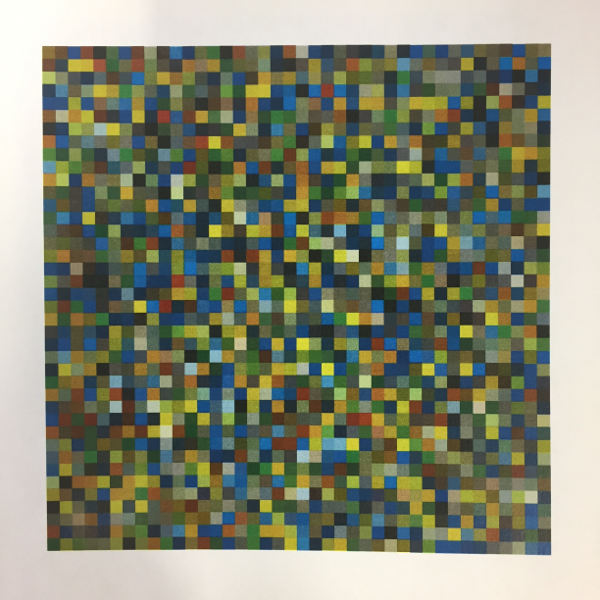
\includegraphics[width=\linewidth]{./rsc/40.png}}
                \end{column}decrypt
                \pause
                \begin{column}{.45\linewidth}
                    \centering{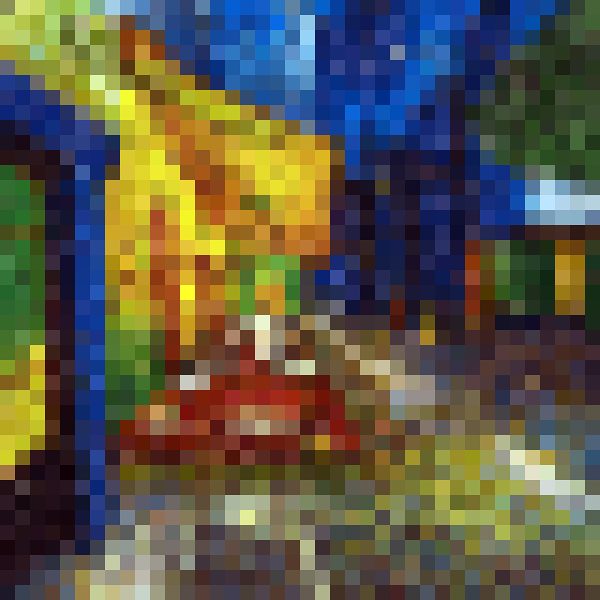
\includegraphics[width=\linewidth]{./rsc/decrypt.png}}
                \end{column}
            \end{columns}
        \end{frame}

    \subsection{Analyse des résultats}

        \begin{frame}
            \frametitle{PSNR découpage en bloc}
            \centering{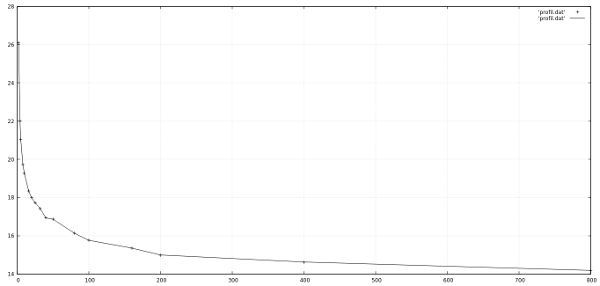
\includegraphics[width=.8\linewidth]{./rsc/psnr_ressemblance.png}}
        \end{frame}

        \begin{frame}
            \frametitle{PSNR lecture et déchiffrement}
            \centering{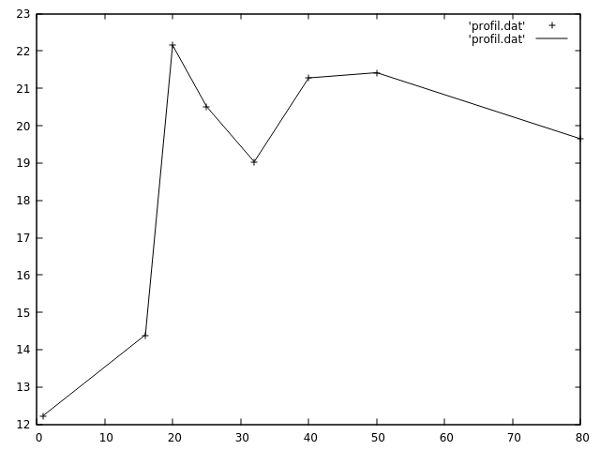
\includegraphics[width=.8\linewidth]{./rsc/psnr_lecture.png}}
        \end{frame}
